

\section*{The Absolute Value Parent Function}

The absolute value parent function is the simplest function that involves an absolute value.

\begin{center}
    \begin{tcolorbox}
        The {\bfseries\itshape absolute value parent function} is written like this:
        \[
            f(x) = |x|
        \]
        where the expression on the right is the absolute value that we talked about 
        in the last lesson.
    \end{tcolorbox}
\end{center}

The graph of the absolute value parent function is shown below.
It looks like a letter {\sffamily\bfseries V}.
You should be able to sketch this graph in homework or on a test.

\begin{center}
    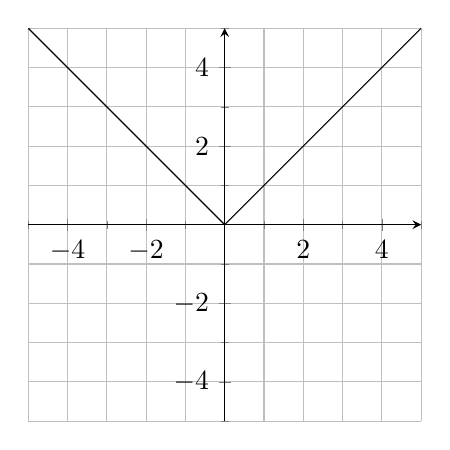
\begin{tikzpicture}
        \begin{axis}[
            width=3in,
            grid=both,
            axis x line = middle,axis y line = middle,
            axis equal image,
            xtick distance = 2, ytick distance = 2,
            xmin = -5, xmax = 5,
            ymin = -5, ymax = 5,
            minor tick num = 1,
            ]
            \addplot[
                no marks,
                mark size = 0.1cm,
                ] expression { abs(x) };
        \end{axis}
    \end{tikzpicture}
\end{center}

For any input, $x$ (positive, zero, or negative), the output $y$ is positive (or zero). 
You can see this, because the graph is completely {\bfseries\itshape above} the $x$-axis,
which means the $y$ values of all the points on the curve are positive (or zero).

\begin{myConceptSteps}{To sketch the graph of the absolute value parent function\dots}
    \myStep{vertex}{Draw a dot at the coordinates $(0,0)$. (This is the \emph{vertex} of the graph.)}
    \myStep{right branch}{
        Starting from the vertex, draw a line with positive slope $1$ going up and to the right
        (rise: {\bfseries\itshape up 1}, run: {\bfseries\itshape right 1}). 
        It goes on forever.
    }
    \myStep{left branch}{
        Starting from the vertex again, draw a line with negative slope $-1$ going up and to the left
        (rise: {\bfseries\itshape up 1}, run: {\bfseries\itshape left 1}). 
        It goes on forever.
    }
\end{myConceptSteps}


\myBlankExample{3in}{
    Sketch the graph of the absolute value parent function,
    $f(x) = |x|$.
}
